\documentclass{article}

\date{01 décembre 2024}
\usepackage[nb-sem=10, auteurs={Kylian Boyet, George Ober, Hugo Vangilluwen, Felix Rondeau}]{../kholles}

\begin{document}
\maketitle

\begin{question_kholle}{Convergence d'une suite si ses sous-suites paires et impaires convergent}
	Soit $(a_{n})_{n \in \N}$ telle que $(a_{2n})_{n \in \N}$ et $(a_{2n+1})_{n \in \N}$ convergent vers la même limite $\ell$.
	Montrons que $a$ converge vers $\ell$.\\
	Soit $\varepsilon>0$. On veut construire un $N \in \N$ tel que $\forall n \geqslant N, \lvert a_{n} - \ell \rvert \leqslant \varepsilon$.\\
	Appliquons la définition de la limite de $(a_{2n})_{n \in \N}$ et $(a_{2n+1})_{n \in \N}$:
	\begin{align*}
		\exists N_{1} \in \N : \forall n \geqslant N_{1}, \lvert a_{2n} - \ell\rvert  \leqslant \varepsilon \\[4pt]
		\exists N_{2} \in \N : \forall n \geqslant N_{2}, \lvert a_{2n+1} - \ell  \rvert \leqslant \varepsilon
	\end{align*}

	\begin{figure}[H]
		\centering
		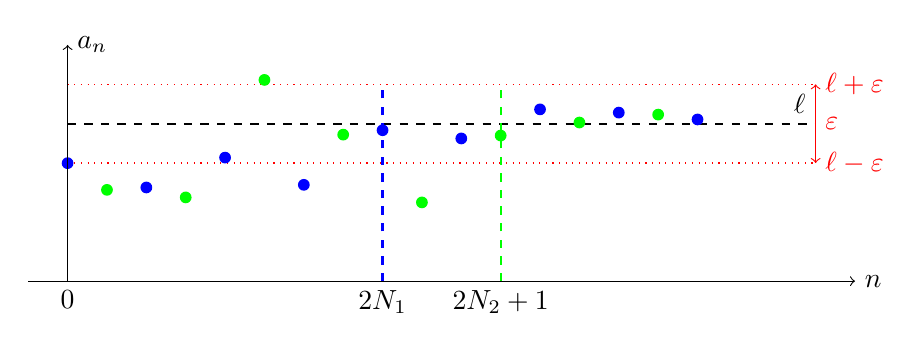
\begin{tikzpicture}
			\draw[thick, dashed] (0.5,2) -- (10,2) node[above left] {$\ell$};

			\draw[dotted, red] (0.5,2.5) -- (10,2.5) node[right] {$\ell + \varepsilon$};
			\draw[dotted, red] (0.5,1.5) -- (10,1.5) node[right] {$\ell - \varepsilon$};

			\foreach \x in {0.5, 1.5, 2.5, 3.5} {
					\node[circle, fill=blue, inner sep=1.5pt] at (\x, {1 + 0.8*rnd}) {}; % Odd terms
				}
			\foreach \x in {1, 2, 3, 4} {
					\node[circle, fill=green, inner sep=1.5pt] at (\x, {1 + 1.8*rnd}) {}; % Even terms
				}

			\node[circle, fill=green, inner sep=1.5pt] at (5, 1) {};

			\node[below] at (4.5,0) {$2N_1$};
			\draw[thick, dashed, blue] (4.5, 0) -- (4.5, 2.5) {};

			\node[below] at (6,0) {$2N_2 + 1$};
			\draw[thick, dashed, green] (6, 0) -- (6, 2.5) {};

			\foreach \x in {4.5, 5.5, 6.5, 7.5, 8.5} {
					\node[circle, fill=blue, inner sep=1.5pt] at (\x, {1.8 + 0.4*rnd}) {};
				}

			\foreach \x in { 6, 7, 8} {
					\node[circle, fill=green, inner sep=1.5pt] at (\x, {1.8 + 0.4*rnd}) {};
				}

			\draw[->] (0,0) -- (10.5,0) node[right] {$n$};
			\node[below] at (0.5,0) {$0$};

			\draw[->] (0.5,0) -- (0.5, 3) node[right] {$a_n$};

			\draw[<->, red] (10,2.5) -- (10,1.5);
			\node[right, red] at (10,2) {$\varepsilon$};

		\end{tikzpicture}
		\caption{Les termes pairs et impairs sont contenus dans un voisinnage de $\ell$ après certains rangs}
	\end{figure}

	\noindent Posons $N = \max(2N_{1}, 2N_{2}+1)$ et vérifions que ce rang convient. \\
	Soit $n \in \N$ tel que $n \geqslant N$.
	\begin{itemize}[label=$\star$]
		\item Si $n$ est pair, $\exists p \in \N :$ $n = 2p$
		      $$
			      n\geqslant N \geqslant 2N_{1} \implies 2p \geqslant 2N_{1} \implies p \geqslant N_{1}
		      $$
		      Donc d'après la définition de la convergence de $(a_{2n})_{n \in \N}$, on a
		      $$
			      \lvert a_{2p} - \ell \rvert  \leqslant \varepsilon \implies \lvert a_{n} - \ell  \rvert  \leqslant \varepsilon
		      $$

		\item Si $n$ est impair, $\exists p \in \N : n = 2p +1$
		      $$
			      n \geqslant N \geqslant 2N_{2}+1 +\implies 2p+1 \geqslant 2N_{2} + 1 \implies p \geqslant N_{2}
		      $$
		      Donc d'après la définition de la convergence de $(a_{2n+1})_{n \in \N}$, on a
		      $$
			      \lvert a_{2p+1} - \ell\rvert  \leqslant \varepsilon \implies \lvert a_{n} - \ell \rvert \leqslant \varepsilon
		      $$
	\end{itemize}
	Donc $\lvert a_{n} - \ell  \rvert\leqslant \varepsilon$
	Donc $a$ tend vers $\ell$.\\[4pt]
	\textbf{Remarque:} Si les deux suites ne convergent pas vers la même limite, comme pour $((-1)^{n})_{n \in \N}$, la suite n'admet pas de limite.
\end{question_kholle}

\begin{question_kholle}{Toute sous-suite d’une suite qui converge vers $\ell\in\C$ converge vers $\ell\in\C$}
	Soient $u$ une suite complexe et $v$ une sous-suite quelconque de $u$.\\
	Par définition d’une sous-suite,
	\[
		\exists \varphi:\N\longrightarrow\N \text{ strictement croissante }: \forall n\in\N, v_{n}=u_{\varphi(n)}
	\]
	Soit $\varepsilon\in\R_{+}^{*}$ fixé quelconque. Appliquons la définition de la convergence de $u$ vers $\ell$ pour $\varepsilon\leftarrow \varepsilon>0$:
	\[
		\exists N\in\N:\forall n\in\N \implies |u_{n}-\ell|\leq \varepsilon
	\]
	Fixons un tel $N$. Soit $n\in\N$ fixé quelconque tel que $n\geq N$. Alors
	\[
		|v_{n}-\ell|=|u_{\varphi(n)}-\ell|\leq \varepsilon
	\]
	car $\varphi$ étant strictement croissante,
	\[
		\varphi(n)\geq n \geq N
	\]
	ce qui permet d’appliquer la définition précédente.

\end{question_kholle}

\begin{question_kholle}
	[Soit $u\in \R ^{\N}$ qui converge vers $\ell \in \R$. \\
		Alors la moyenne arithmérique des $n\in \N$ premiers termes (appelée moyenne de Césarò) converge vers $\ell$.]
	{Théorème de Césarò}

	Soient $u$ une telle suite, $\varepsilon \in \R ^*_+$ et $\ell \in \R$ ladite limite de $u$.\\
	Appliquons la définition de la convergence de $u$ pour $\varepsilon \gets \frac{\varepsilon}{2}$ :
	\[
		\exists N \in \N \ : \ \forall n \in \N , \ n\geq N \ \implies \ |u_n - \ell | \leq \frac{\varepsilon}{2}.
	\]
	Fixons un tel $N$. Posons
	\[
		\omega = \sum_{k=0}^{N-1} |u_k - \ell | \in \R
	\]
	Soit $n\in \N$ tel que $n \geq N$. Calculons :
	\[
		\left| \frac{1}{n} \sum_{k=0}^{n-1}u_k - \ell \right| = \left| \frac{1}{n} \left( \sum_{k=0}^{n-1}u_k - n\ell \right) \right|  = \left| \frac{1}{n} \sum_{k=0}^{n-1}(u_k - \ell)  \right| \leq \frac{1}{n} \underset{= \ \omega \in \R}{\underbrace{\sum_{k=0}^{N-1}|u_k - \ell|}} + \frac{1}{n} \underset{\leq \ \frac{\varepsilon}{2}}{\underbrace{\sum_{k=N}^{n}|u_k - \ell|}} \leq \frac{\omega}{n} + \underset{\leq \ \frac{\varepsilon}{2}}{\underbrace{\frac{\varepsilon}{2n}}}.
	\]
	Ces majorations sont issues de l'inégalité triangulaire et de la convergence de $u$.\\
	De plus, comme la suite $(v_n) _{n\in \N} = \left( \frac{\omega}{n} \right) _{n\in \N}$ converge vers $0$, on écrit sa définition pour $\varepsilon \gets \frac{\varepsilon}{2}$ :
	\[
		\exists N' \in \N \ : \ \forall n \in \N , \ n\geq N' \ \implies \ |v_n| \leq \frac{\varepsilon}{2}.
	\]
	On fixe un tel $N'$ et on pose $\Lambda = \max{(N, N')}$ qui a bien un sens car $\{N, \ N'\}$ est une partie finie de $\N$.
	De la même manière qu'auparavant, pour $n\in \N$ tel que $n \geq \Lambda$, on a :
	\[
		\left| \frac{1}{n} \sum_{k=0}^{n-1}u_k - \ell \right| \leq \underset{\leq \ \frac{\varepsilon}{2}}{\underbrace{\frac{\omega}{n}}} + \frac{\varepsilon}{2} \leq \varepsilon.
	\]
	C'est le théorème souhaité.
\end{question_kholle}

\begin{question_kholle}
	[Soit $u \in \R^\N$ une suite monotone :
	{\begin{enumerate}
		\item Si $u$ est croissante
		      \begin{enumerate}[label=($\roman*$)]
			      \item Soit $u$ est majorée, et dans ce cas, $\lim u = \sup\{ u_k | k \in \N \}$
			      \item Soit $u$ n'est pas bornée, et dans ce cas, $u$ diverge vers $+\infty$.
		      \end{enumerate}
		\item Si $u$ est décroissante :
		      \begin{enumerate}[label=($\roman*$) Soit, leftmargin=4em]
			      \item $u$ est minorée, et dans ce cas, $\lim u = \inf\{ u_k | k \in \N \}$
			      \item $u$ n'est pas bornée, et dans ce cas, $u$ diverge vers $-\infty$.
		      \end{enumerate}
	\end{enumerate} }]
	{Théorème de la convergence monotone}

	Soit $u \in \R^\N$ monotone fq.

	\begin{enumerate}
		\item Supposons que $u$ est croissante.
		      \begin{enumerate}[label=($\roman*$)]
			      \item Supposons que $u$ est majorée. \\
			            Alors $\exists M \in \R : \forall n \in \N, u_n \leqslant M$. Fixons un tel M. \\
			            $\Omega = \{ u_k | k \in \N \}$ est \begin{itemize}
				            \item une partie de \R
				            \item non vide car $u_0$ y appartient
				            \item majorée par M
			            \end{itemize}
			            donc elle admet un borne supérieure et notons-la $\sigma$. \\
			            Soit $\epsilon \in \R_+^*$ fq. \\
			            $\sigma - \epsilon < \sigma$ donc $\sigma - \epsilon$ ne majore pas $\Omega$. Donc $\exists N \in \N : u_N > \sigma - \epsilon$. Fixons un tel N. \\
			            Soit $n \in \N$ fq tq $n \geqslant N$. \\
			            Alors $u_n \underset{\text{par croissant de u}}{\geqslant} u_N \geqslant \sigma - \epsilon$ et $u_n \underset{\text{par défintion de }\sigma}{\leqslant} \sigma$. \\
			            Ainsi,
			            \begin{equation*}
				            \begin{aligned}
					            \sigma - \epsilon \leqslant u_n \leqslant \sigma
					             & \implies - \epsilon \leqslant u_n - \sigma \leqslant 0 \\
					             & \implies | u_n - \sigma | \leqslant \epsilon
				            \end{aligned}
			            \end{equation*}
			            Donc $u_n \arrowlim{n}{+\infty} \sigma$.

			      \item Supposons que $u$ n'est pas bornée. \\
			            Soit $A \in \R$ fq. \\
			            $u$ n'est pas bornée donc $\exists N \in \N : u_N > A$. \\
			            Or $u$ est croissante donc $\forall n \in \N, n \geqslant N \implies u_n \geqslant A$. \\
			            Donc $u_n \arrowlim{n}{+\infty} +\infty$.
		      \end{enumerate}

		\item Supposons que $u$ est décroissante. \\
		      Il suffit dans la preuve ci-dessus de remplacer les inégalités inférieures par des inégalités supérieures et inversement et d'utiliser la notion de borne inférieure plutôt que de borne supérieure.
		      \begin{enumerate}[label=($\roman*$)]
			      \item Si $u$ est minorée, $u_n \arrowlim{n}{+\infty} \inf\{u_k|k\in\N\}$.
			      \item Si $u$ n'est pas bornée, $u_n \arrowlim{n}{+\infty} -\infty$.
		      \end{enumerate}
	\end{enumerate}
\end{question_kholle}

\begin{question_kholle}
	[Soient $(u,v) \in \R^{\N}$ : \\
	{\begin{enumerate}[label=($\roman*$)]
		\item Si
		      \[
			      \exists N \in \N : \forall n \in \N, n \geqslant N \implies u_{n} \geqslant 0  \quad \text{ et \quad $u$ converge}
		      \]
		      Alors $\lim u \geqslant 0$
		\item Si
		      \[
			      \exists N \in \N : \forall n \in \N, n \geqslant N \implies u_{n} \leqslant v_{n} \quad  \text{ et \quad $u$ et $v$ convergent}
		      \]
		      Alors $\lim u \leqslant \lim v$
	\end{enumerate}}
	]
	{Théorème de passage à la limite dans une inégalité.}
	~\smallbreak
	\begin{enumerate}[label=($\roman*$)]
		\item L'hypothèse $\exists N \in \N : \forall n \in \N, n \geqslant N \implies u_{n} \geqslant 0$ permet d'affirmer que $u$ et $|u|$ coïncident à partir d'un certain rang. \\
		      Par ailleurs, la convergence de $u$ et la continuité de $|\cdot|$ sur $\R$ donc en $\lim u$ donnent $|u|$ converge vers $|\lim u|$. \\
		      Le caractère asymptotique de la limite permet de conclure que $u$ et $|u|$ ont la même limite. \\
		      Donc $\lim u = |\lim u| \geqslant 0$.
		\item $\exists N \in \N : \forall n \in \N, n \geqslant N \implies u_{n} \leqslant v_{n} \implies v_{n} - u_{n} \geqslant 0$ \\
		      $u$ et $v$ convergent $\implies v-u$ converge vers $\lim v - \lim u$. \\
		      On applique $(i)$ pour $u \leftarrow v - u$, autorisé car $u \text{ et }v$ convergent. \\
		      On obtient $\lim v - \lim u \geqslant 0$ d'où $\lim u \leqslant \lim v$.
	\end{enumerate}
\end{question_kholle}


\begin{question_kholle}{Théorème d’existence de la limite par encadrement}
	\hfill\\
	\textbf{Résultat préliminaire: théorème «~sans nom~».}\\
	\textit{Théorème: } Soient $u\in\K^{\N}, \ell\in\K$ et $(\varepsilon_{n})_{n\in\N}\in\R^{\N}$. Si
	\[
		\begin{cases}
			\exists N\in\N: \forall n\in\N, n\geq N \implies |u_{n}-\ell|\leq \varepsilon_{n} \\
			\lim \varepsilon=0
		\end{cases}
	\]
	alors la suite $u$ converge vers $\ell$.\\[4pt]
	\textit{Démonstration: }
	Soit $\delta\in\R_{+}^{*}$ fixé quelconque.\\
	Appliquons la définition de la convergence de $(\varepsilon_{n})$ vers 0 pour $\varepsilon\leftarrow \delta>0$:
	\[
		\exists N_{0}\in\N: \forall n\in\N, n\geq N_{0}\implies |\varepsilon_{n}-0|\leq \delta
	\]
	Fixons un tel $N_{0}$. Soit $N$ tel que
	\[
		\forall n\in\N, k\geq N \implies  |u_{n}-\ell|\leq \varepsilon
	\]
	Posons $N_{1}=\max \left\{N_{0}, N\right\}$. Soit $n\in\N$ fixé quelconque tel que $n\geq N_{1}$. alors
	\[
		|u_{n}-\ell|\leq \varepsilon_{n} \leq |\varepsilon_{n}| \leq \delta
	\]
	ce qui conclut la preuve.\\[5pt]

	\noindent\textbf{Théorème d’existence de la limite par encadrement}
	Soient $(u,v,w)\in{\R^{\N}}^{3}$ trois suites. Supposons
	\[
		\begin{cases}
			\exists N\in\N:\forall n\in\N, n\geq N \implies u_{n}\leq v_{n}\leq w_{n} \\
			\text{$u$ et $w$ convergent vers $u_{\infty}$ et $w_{\infty}$}            \\
			u_{\infty} = w_{\infty}
		\end{cases}
	\]
	En retranchant $u_{n}$,
	\[
		\forall n\in\N, 0\leq v_{n}-u_{n}\leq w_{n}-u_{n}
	\]
	donc
	\[
		|v_{n}-u_{n}|\leq w_{n}-u_{n}
	\]
	et de plus, $w$ et $u$ convergent vers $\ell-\ell=0$ si bien que le théorème sans nom s’applique pour $a\leftarrow v-u$, $\ell\leftarrow 0$ et $b\leftarrow w-u$ et établit la convergence de $v-u$ vers 0. Ainsi, comme $u$ converge vers $\ell$, la combinaison linéaire de suites convergentes $v-u+u$ converge vers $0+\ell=\ell$, si bien que la suite $v$ converge vers $\ell$.
\end{question_kholle}


\begin{question_kholle}
	[Soient $u$ et $v$ deux suites réelles adjacentes. Alors $u$ et $v$ convergent et ont la même limite.]
	{Théorème des suites adjacentes}

	Soient $u$ et $v$ de telles suites. Quitte à inverser les rôles desdites suites, prenons $u$ croissante et $v$ décroissante. \\
	On a donc :
	\[
		\forall n \in \N, \ (u_n \leq v_n \leq \underset{\in \R}{\underbrace{v_0}}) \wedge (\underset{\in \R}{\underbrace{u_0}}\leq  u_n \leq v_n),
	\]
	car la monotonie des suites induit ces inégalités. D'après le théorème de limite monotone, $u$ étant croissante et majorée elle converge, $v$ étant décroissante et minorée elle converge. \\
	Il s'en suit que par définition des suites adjacentes :
	\[
		0 \ = \lim_{n \to +\infty} (u_n - v_n) \ \underset{u,v \ \text{ convergent}}{\underbrace{=}} \ \lim_{n \to +\infty} u_n - \lim_{n \to +\infty} v_n.
	\]
	Ainsi, $\lim u = \lim v$.
\end{question_kholle}


\begin{question_kholle}
	[Toute suite bornée réelle admet une sous-suite convergente. \\
		L'ensemble des valeurs d'adhérence d'une suite réelle bornée est non vide.]
	{\emph{Facultative} Théorème de Bolzano-Weierstrass}

	Soit $u \in \R^\N$ fixée quelconque bornée. \\
	Alors $\exists M \in \R_+ : \forall n \in \N, |u_n| \leqslant M$.

	Construisons une suite de segments dans $[-M;M]$ de plus en plus petits par dichotomie. \\
	Posons $a_0 = -M$, $b_0 = M$ et définissons les suites $c$ et $I$ pour tout $n$ dans \N par $c_n = \frac{a_n + b_n}{2}$ et $I_n = [a_n;b_n]$. \\

	\noindent Soit $n\in \N$ fq.
	Supposons $a_n \text{ et } b_n$ construits et $\{ k \in \N \;|\; u_k \in I_n \}$ infini.
	Construisons les termes d'indices $n+1$. \\
	Posons $\left| \begin{array}{lcr}
			I_n^- & = & \{ k \in \N \;|\; u_k \in [a_n;c_n] \} \\
			I_n^+ & = & \{ k \in \N \;|\; u_k \in [c_n;b_n] \} \\
		\end{array} \right.$ \\
	Nous avons $I_n^- \cup I_n^+ = \{ k \in \N \;|\; u_k \in I_n \}$ donc $I_n^-$ ou $I_n^+$ est infini.

	\begin{itemize}
		\item Si $I_n^-$ est infini, posons $\left| \begin{array}{lcl}
				      a_{n+1} & = & a_n \\
				      b_{n+1} & = & c_n
			      \end{array} \right.$ \\
		      Ainsi $\{ k \in \N \;|\; u_k \in I_{n+1} \} = I_n^-$ est infini.
		\item Si $I_n^+$ est infini, posons $\left| \begin{array}{lcl}
				      a_{n+1} & = & c_n \\
				      b_{n+1} & = & b_n
			      \end{array} \right.$ \\
		      Ainsi $\{ k \in \N \;|\; u_k \in I_{n+1} \} = I_n^+$ est infini.
	\end{itemize}
	\bigbreak

	\noindent Étudions la suite $\left(I_n\right)_{n\in\N}$.
	\begin{itemize}
		\item Nous avons toujours $a_n \leqslant b_n$ donc $\forall n \in \N, I_n \neq \emptyset$
		\item Par construction, $\forall n \in \N, I_{n+1} \subset I_n$
		\item $ |I_{n+1}| = |a_{n+1}-b_{n+1}| = \frac{1}{2} |a_n-b_n| = \frac{1}{2} |I_n| $
		      donc la suite des cardinaux est une suite géométrique de raison $\nicefrac{1}{2}$.
		      Donc $|I_n| \arrowlim{n}{+\infty} 0$.
	\end{itemize}
	Donc, d'après le théorème des segments emboîtés, $\exists ! l\ell \in \R : \underset{n\in\N}{\bigcap} I_n = \{\ell\}$. Fixons un tel $\ell$. \\

	Construisons maintenant une extractrice $\varphi$ de $u$. \\
	Posons $\varphi(n) = 0$. \\
	Soit $n \in \N$ fq. Supposons $\varphi(n)$ construite.
	\begin{equation*}
		\varphi(n+1) = \min\{ k \in \N | u_k \in I_{n+1} \wedge k > \varphi(n) \}
	\end{equation*}
	$\varphi(n+1)$ est bien définie car $\{ k \in \N | u_k \in I_{n+1} \}$ est une partie de \N non bornée (car infinie). \\

	\noindent Ainsi, nous avons construit $\varphi : \N \rightarrow \N$ strictement croissante. Nous pouvons extraire une sous-suite de $u$. Or $\forall n \in \N, u_{\varphi(n)} \in I_n$ donc
	\begin{equation*}
		\forall n \in \N, \quad
		\underbrace{a_n}_{ \arrowlim{n}{+\infty} \ell } \leqslant u_{\varphi(n)} \leqslant \underbrace{b_n}_{ \arrowlim{n}{+\infty} \ell }
	\end{equation*}
	Donc, d'après le théorème d'existence de limite par encadrement, $u_{\varphi(n)} \arrowlim{n}{+\infty} \ell$. \\
	Ainsi $\ell \in L_u$.
\end{question_kholle}


\begin{question_kholle}
	[Soit $u$ une suite bornée. $u$ converge si et seulement si il existe $\ell \in \mathbb{K}$ tel que $L(u)$ est le singleton $\ell$ ]
	{\emph{Facultative} Caractérisation de la convergence par l'unicité d'une valeur d'adhérence pour une suite bornée.}
	Traitons le cas réel, celui sur \C est à adapter sans peine.\\
	Supposons que $u$ converge et posons $\lim u =\ell \in \R  $. Toutes les sous-suites de $u$ convergent vers $\ell$ donc $L(u)=\{\ell \}$. \\
	Supposons maintenant qu'il existe un unique $\ell \in \R$ tel que $L(u) = \{ \ell \}$. Par l'absurde, supposons que $u$ ne converge pas vers $\ell$, c'est-à-dire :
	\[
		\exists \varepsilon \in \R ^* _+ \ : \ \forall N \in \N, \ \exists n \in \N \ : \ n\geq N \text{ et } |u_n - \ell | > \varepsilon.
	\]
	Fixons un tel $\varepsilon$. \\
	%\textbf{Etape 1} : \textit{Construction d'une sous-suite de $u$ dont les termes sont $\varepsilon$-éloignés de $\ell$.} \\
	Posons $\varphi (0) = \min{ \{ k\in \N \ | \ |u_k - \ell| > \varepsilon \} }$, ce qui a du sens car c'est une partie non-vide de $\N$. Posons ensuite $\varphi (1) = \min{ \{ k\in \N \ | \ |u_k - \ell| > \varepsilon, \ \varphi(0) < k \} } $, ce qui a du sens pour les mêmes raisons. On construit en itérant ce procédé $\varphi (n)$ tel que :
	\[
		\forall n \in \N, \ \varphi(n+1) = \min{ \{ k\in \N \ | \ |u_k - \ell| > \varepsilon, \ \varphi(n) < k \} }.
	\]
	De cette manière, nous venons de construire une extractrice telle que :
	\[
		\forall n \in \N, \ |u_{\varphi(n)} - \ell| > \varepsilon.
	\]
	Par hypothèse $u$ est bornée, donc il existe $M\in \R _+$ tel que :
	\[
		\forall n \in \N, \ |u_n| \leq M,
	\]
	donc pour tout $n$ dans $\N$, $|u_{\varphi(n)}| \leq M$, donc $(u_{\varphi(n)})_{n\in \N}$ est bornée. \\
	Par le théorème de Bolzano-Weierstrass, il existe $\psi$ une extractrice et $\ell ' \in \R$, avec $\varphi \circ \psi$ qui est aussi une extractrice par composition d'applications strictement croissantes, donc$(u_{\varphi \circ \psi (n)})_{n\in \N}$ est une sous-suite de $u$ et $\ell ' \in L(u) = \{ \ell \}$.\\
	Par ailleurs, pour tout $n$ dans $\N$ :
	\[
		\underset{\xrightarrow[n\to +\infty]{}|\ell' -\ell|}{\underbrace{|u_{\varphi \circ \psi (n)} - \ell|}} > \varepsilon,
	\]
	donc en passant à la limite dans l'inégalité on a pour tout $n$ dans $\N$, $|\ell ' - \ell | \geq \varepsilon > 0$, ce qui n'est pas possible car $\ell$ est la seule valeur d'adhérence possible et ici la différence n'est pas nulle.
\end{question_kholle}



\pagebreak
\begin{question_kholle}
	[\noindent Soient $(A, B) \in \mathcal{P}(\R)^2$ fq. \\
		\textit{Définition de la densité}
		\begin{align}
			A \text{ est dense dans } B
			\text{ si } \left\{ \begin{array}{ll}
				                    A \subset B \\
				                    \mathrm{et} \\
				                    \forall (u,v) \in \R^2, B \cap {]}u;v{[} \neq \emptyset \implies A \cap  {]}u;v{[} \neq \emptyset
			                    \end{array} \right.
		\end{align}
		\textit{Caractérisation de la densité par les $\varepsilon$}
		\begin{align}
			A \text{ est dense dans } B
			\iff \left\{ \begin{array}{ll}
				             A \subset B \\
				             \mathrm{et} \\
				             \forall b \in B, \forall \varepsilon \in \R_+^*, \exists a \in A: |b-a|< \varepsilon
			             \end{array} \right.
		\end{align}
	]
	{[Non demandée] Caractérisation de la densité d’une partie $A$ de \R dans une partie $B$ de \R la contenant avec des $\varepsilon$.}

	\textit{Montrons la caractérisation de la densité}\\
	\emph{Sens Direct} Supposons $A$ dense dans $B$
	\begin{itemize}[label=\textemdash]
		\item Par déf $A \subset B$
		\item Soit $b \in B$ et $\varepsilon \in \R_+^*$ fq

		      Appliquons le (ii) de la déf de Densité pour $u \leftarrow b - \varepsilon$ et $v \leftarrow b + \varepsilon$
		      $$B \cap ]b - \varepsilon, b + \varepsilon[ \neq \emptyset \implies A \cap ]b - \varepsilon,  b + \varepsilon[ \neq \emptyset$$
			      Or, $B \cap ]b - \varepsilon, b + \varepsilon[ \neq \emptyset$ est vraie
				      donc $A \cap ]b - \varepsilon,  b + \varepsilon[ \neq \emptyset$

				      Ce qui permet de choisir $a \in A \cap ]b - \varepsilon,  b + \varepsilon[$.
				      Un tel $a$ vérifie $a \in A$ et $a \in ]b - \varepsilon,  b + \varepsilon[ \iff |b-a| < \varepsilon$
	\end{itemize}
	\bigbreak
	\noindent \emph{Sens réciproque} Supposons $\left\{\begin{array}{ll} A \subset B \\\mathrm{et}\\ \forall b \in B, \forall \varepsilon \in \R_+^*, \exists a \in A: |b-a|< \varepsilon \end{array}\right.$

	\begin{itemize}
		\item On a donc $A \subset B$
		\item Soient $(u, v) \in \R^2$ fq tq $B \cap ]u, v[ \neq \emptyset$

						      Soit $b \in B \cap ]u, v[$ fq.
						      Appliquons l'hypothèse pour $b\leftarrow b$ et $\varepsilon \leftarrow \min\{v - b, b - u\}$, qui est autorisé $v-b$ et $b-u$ sont positifs

						      Donc $\exists a \in A: | b - a| < \varepsilon $

						      Fixons un tel a, alors:
						      $$
							      b-\varepsilon < a < b + \varepsilon
						      $$

						      Donc $$
							      \left\{\begin{array}{ll}
								      a < b + \varepsilon = b + \underbrace{\min\{v - b, b - u\}}_{\leqslant v - b} \leqslant b + v - b = v \\ \mathrm{et}\\
								      a > b - \varepsilon = b - \underbrace{\min\{v - b, b - u\}}_{\leqslant b - u} \geqslant b - (b - u) = u
							      \end{array}\right.
						      $$

						      Donc $a \in ]u, v[$.
	\end{itemize}
	Donc $A \cap ]u, v[ \neq \emptyset$

\end{question_kholle}

\begin{question_kholle}
	[\begin{equation}
			\forall (a, b) \in \R \times \R^*,
			\exists ! (q, r) \in \Z \times \R :
			\left\{ \begin{matrix}
				a = b q + r \\
				r \in [0;|b|[
			\end{matrix} \right.
		\end{equation}]
	{[Non demandée] Théorème de la division pseudo-euclidienne dans \R}

	\textit{Unicité} \;
	Soient deux tels entiers $(a,b) \in \R^2$ et deux couples $((q,r),(q',r')) \in \left(\Z \times \R\right)^2$ tels que
	\begin{equation*}
		\left\{ \begin{matrix}
			a = b q + r \\
			r \in [0;|b|[
		\end{matrix} \right.
		\qquad
		\left\{ \begin{matrix}
			a = b q' + r' \\
			r' \in [0;|b|[
		\end{matrix} \right.
	\end{equation*}
	Directement,
	\[
		b(q-q') = r'-r,
	\]
	mais comme $-|b| < r' - r < |b|$, il vient en divisant par $|b|$ l'inégalité précédente :
	\[
		-1 < q - q' < 1,
	\]
	puisque $q$ et $q'$ sont dans $\Z$ leur différence est obligatoirement $0$, ainsi $q = q'$ ce qui implique $ r= r'$ et donc on a unicité de ladite écriture de $a$.
	\newline
	\\
	\textit{Existence} \; Posons pour $b > 0$, $\Omega = \{ k\in \Z  \ | \ kb \leqslant a \}$
	\begin{itemize}
		\item $\Omega \subset \Z$
		\item non-vide car $-|a| \in \Omega$ ($\Z$ archimédien suffit \ldots)
		\item $\Omega$ est majoré par $|a|$ car supposons, par l'absurde, que $\exists k \in \Omega : k > |a|$, alors $kb > |a|b > a$ ce qui contradiction avec la définition d'$\Omega$.
	\end{itemize}
	Donc $\Omega$ admet un plus grand élément, notons-le $q$. \\
	Posons $r = a - bq$. Par construction, $a = bq + r$ et comme $q = \max \Omega$ et $r \in \R$.
	\\
	Par suite, $q \in \Omega$ donc $bq \leqslant a$ d'où $0 \leqslant r$. Et $q = \max \Omega$ donc $b(q+1) > a$ d'où $b > r$, c'est-à-dire, $r \in [ 0, |b| [$.

	Si $b < 0$, il suffit de prendre $q \leftarrow -q$ dans la preuve précédente.C'est donc l'existence de ladite écriture de $a$.
\end{question_kholle}

\begin{question_kholle}
	{[Non demandée] \Q est dense dans \R et $\R \setminus \Q$ est aussi dense dans \R}

	Soit $x \in \R$ fq.
	Posons $\forall n \in \N, a_n = \frac{\lfloor2^n x\rfloor}{2^n}$. \\
	Soit $n \in \N$ fq. \\
	\begin{itemize}
		\item $a_n \in \Q$ car $\lfloor2^n x\rfloor \in \Z$ et $2^n \in \N$.
		\item \begin{equation*}
			      a_n = \frac{\lfloor2^n x\rfloor}{2^n}
			      \implies \frac{2^n x - 1}{2^n} \leqslant a_n \leqslant \frac{2^n x}{2^n}
			      \implies x - \frac{1}{2^n} \leqslant a_n \leqslant x
		      \end{equation*}
		      Or $\nicefrac{1}{2^n} \arrowlim{n}{+\infty} 0$ donc d'après le théorème d'existence de limite par encadrement, \\ $a_n \arrowlim{n}{+\infty} x$.
	\end{itemize}
	Donc d'après la caractérisation séquentielle de la densité, \Q est dense dans \R.
	\bigbreak

	\noindent Soit $x \in \R$ fq. \\
	Alors $x + \sqrt{2} \in \R$.
	D'après la démonstration précédente, $\exists b \in \Q^\N : b_n \arrowlim{n}{+\infty} x + \sqrt{2}$. \\
	Fixons un telle suite $b$.
	Considérons $c = b - \sqrt{2}$. \\
	Soit $n \in \N$ fq.
	\begin{itemize}
		\item $c_n \in \R\setminus\Q$ car $b_n \in \Q$ et $\sqrt{2} \in \R \setminus \Q$.
		\item \begin{equation*}
			      \left. \begin{matrix}
				      b_n \arrowlim{n}{+\infty} x + \sqrt{2} \\
				      c_n = b_n - \sqrt{2}
			      \end{matrix} \right\}
			      \implies c_n \arrowlim{n}{+\infty} x
		      \end{equation*}
	\end{itemize}
	Donc d'après la caractérisation séquentielle de la densité, $\R\setminus \Q$ est dense dans \R.
\end{question_kholle}

\begin{question_kholle}[
		Soit u $\in \K ^ \N, (\ell_1, \ell_2) \in \K ^2$
		Si u converge vers $\ell_1$ et $\ell_2$, alors $\ell_1 = \ell_2$
	]{[Non demandée] Preuve de l'unicité de la limite d'une suite convergente}
	Par l'absurde, supponsons que $u$ converge vers $\ell_1$ et $\ell_2$, et $\ell_1 \neq \ell_2$.
	On prendra $\varepsilon_0 = \varepsilon_1 = \varepsilon_2$ assez petit pour que les tubes soient disjoints.\\
	Posons donc $\varepsilon_0 = \frac{|\ell_1 - \ell_2|}{3}$
	\begin{itemize}
		\item Appliquons la définition de la convergence de u vers $\ell_1$, pour $\varepsilon \leftarrow \varepsilon_0$, ce qui est autorisé car $\varepsilon_0 \in \R_+^*$
		      \begin{equation}\label{eq:1}
			      \exists N_1 \in \N : \forall n \in \N, n \geqslant N_1 \implies |u_n - \ell_1| \leqslant \varepsilon_0
		      \end{equation}
		      \begin{equation}\label{eq:2}
			      \exists N_2 \in \N : \forall n \in \N, n \geqslant N_2 \implies |u_n - \ell_2| \leqslant \varepsilon_0
		      \end{equation}
		      Fixons de tels $N_1$ et $N_2$.
		\item Posons $n_0 = N_1 + N_2$
		      \begin{itemize}
			      \item $n_0 \geqslant N_1$, donc (\ref{eq:1}) s'applique: $|u_{n_0} - \ell_1| \leqslant \varepsilon_0$
			      \item $n_0 \geqslant N_2$, donc (\ref{eq:2}) s'applique: $|u_{n_0} - \ell_2| \leqslant \varepsilon_0$
		      \end{itemize}
		\item \begin{align*}
			      |\ell_1 - \ell_2| & = |\ell_1 - u_{n_0} + u_{n_0} - \ell_2|                                                                                         \\
			                        & \leqslant \underbrace{|\ell_1 - u_{n_0}|}_{\leqslant \varepsilon_0} + \underbrace{|u_{n_0} - \ell_2|}_{\leqslant \varepsilon_0} \\
			                        & \leqslant 2 \frac{|\ell_1 - \ell_2|}{3}                                                                                         \\
			      \implies 1        & \leqslant \frac 2 3
		      \end{align*}
		      Contradiction
	\end{itemize}
\end{question_kholle}
\begin{question_kholle}[{
				Soient $(x, y) \in \R^2$ tels que $x \leqslant y$. $$[x, y] = \{z \in \R \mid x \leqslant z \leqslant y \} = \{tx + (1-t)y \mid t \in [0, 1]\}$$
			}]{[Non demandée] Description d'un segment de la droite réelle par les barycentres à coefficients positifs.}
	Le résultat est immédiat pour $x = y$ : $\forall t \in [0, 1], xt+(1-t)x = xt - xt +x =x = y$

	Supposons que $x <y$. On procède par double inclusion.
	\begin{itemize}[label=$\star$]
		\item Soit $z \in \{ xt+(1-t)y \mid t \in [0, 1] \}$.

		      $\exists t \in [0, 1] : z = xt+(1-t)y$

		      Puisque $t \in [0, 1]$, $t \geqslant 0$ et $1-t \geqslant 0$.
		      Donc

		      \begin{align*}
			      x < y \implies x\leqslant y & \underset{ \substack{t \geqslant 0                  \\1-t \geqslant 0} }{ \implies } \left\{ \begin{array}{ll}
				      tx \leqslant ty \\
				      (1-t)x \leqslant (1-t)y
			      \end{array}\right. \\
			                                  & \implies \left\{ \begin{array}{ll}
				                                                     tx + (1-t)y \leqslant ty + (1-t) y \\
				                                                     tx + (1-t)x  \leqslant tx + (1-t)y
			                                                     \end{array}\right. \\
			                                  & \implies \left\{ \begin{array}{ll}
				                                                     z \leqslant y \\
				                                                     x \leqslant z
			                                                     \end{array}\right.                 \\
			                                  & \implies z \in[x, y]
		      \end{align*}



		\item Réciproquement, soit $z \in[x, y]$. Cherchons le $t\in[0, 1]$ tel que $tx + (1-t)y = z$.

		      $$
			      tx + (1-t)y = z \iff t(x-y) = z-y \iff t = \frac{z-y}{x-y} = \frac{y-z}{y-x} \text{ (autorisé car }x<y \implies x-y \neq 0 \text{)}
		      $$

		      Vérifions si ce $t$ convient : posons $t = \frac{y-z}{y-x}$.
		      \begin{itemize}[label=$\bullet$]
			      \item Vérifions d'abord que $t \in [0,1]$

			            $$
				            x\leqslant z \leqslant y
				            \implies x-y \leqslant z-y \leqslant 0 \implies y-x\geqslant y-z \geqslant 0 \implies 1 \geqslant \frac{y-z}{y-x} \geqslant 0 \implies 0\leqslant t \leqslant 1
			            $$
			      \item Calculons
			            $$
				            tx+(1-t)y = \frac{y-z}{y-x} x + \left( 1- \frac{y-z}{y-x} \right)y = \frac{y-z}{y-x}x + \frac{z-x}{y-x}y = \frac{yx-zx+zy - xy}{y-x} =  z
			            $$
			            Donc ce $t$ convient.
		      \end{itemize}
		      Donc $z \in \{ xt+(1-t)y \mid t \in [0, 1] \}$.
	\end{itemize}
	Donc $\{ xt+(1-t)y \mid t \in [0, 1] \} = [x, y]$.
\end{question_kholle}
\begin{question_kholle}{[Non demandée] Une suite convergente est bornée}

	Soit $u \in \mathbb{K}^{\mathbb{N}}$ convergente.
	Posons $\ell = \lim u$
	Appliquons la définition de la convergence pour $\varepsilon \leftarrow 1$
	$$
		\exists N_{1}\in \mathbb{N}: \forall n \in \mathbb{N}, n \geqslant N_{1} \implies |u_{n}-\ell| \leqslant 1
	$$
	Fixons un tel $N_{1}$
	Posons alors $M = \max\left\{ |u_{0}|, |u_{1}|, |u_{2}| \dots |u_{N_{1}}|, |\ell|+1 \right\}$, qui est bien défini, car toute partie finie, non vide d'un ensemble totalement ordonné (ici $(\mathbb{R}, \leqslant)$) admet un pgE.

	Soit $n \in \mathbb{N}$ fq.
	\begin{itemize}
		\item Si $n \in [[0, N_{1}]], |u_{n}| \in \left\{ |u_{0}|, |u_{1}|, |u_{2}| \dots |u_{N_{1}}|, |\ell|+1 \right\}$ donc $|u_{n}| \leqslant M$
		\item Sinon,
	\end{itemize}

	\begin{align*}
		n> N_{1} & \implies |u_{n} - \ell| \leqslant 1              \\
		         & \implies |u_{n}| - |\ell| \leqslant 1            \\
		         & \implies |u_{n}| \leqslant 1+ |\ell| \leqslant M
	\end{align*}

	Ainsi, $\forall n \in \mathbb{N}, |u_{n}| \leqslant M$.
\end{question_kholle}
\begin{question_kholle}[{Soit $A \in \mathcal{P}(\R)$ non vide et majorée. Soit $\sigma \in \R$
				$$
					\sigma = \sup A \iff \left\{ \begin{array}{ll}
						\sigma \in M(A) \\
						\exists (a_{n})_{n \in \N} \in A^{\N} : \lim_{n \to +\infty} a_n = \sigma
					\end{array}\right.
				$$
			}]{[Non demandée] Caractérisation séquentielle de la borne supérieure}
	\begin{itemize}[label=$\star$]
		\item Supposons que $\sigma = \sup A$.
		      \begin{itemize}[label=$\bullet$]
			      \item Par définition d'une borne sup, $\sigma \in M(A)$.
			      \item Soit $n \in \N$. Appliquons la caractérisation de la borne sup par les epsilon pour $\varepsilon \leftarrow \frac{1}{2^{n}}$.
			            $\exists c \in A : \sigma - \frac{1}{2^{n}} < c \leqslant \sigma$.
			            Fixons un tel $c$ et notons le $a_{n}$. En relâchant le caractère fixé de $n$, on a crée la suite $(a_{n})_{n \in \N}$ telle que
			            $$
				            \forall n \in \N, \sigma - \frac{1}{2^{n}} < a_{n}\leqslant \sigma
			            $$
			            Cette suite converge vers $\sigma$ par encadrement.
		      \end{itemize}
		\item Réciproquement, supposons que $\sigma \in M(A)$ et qu'il existe une suite $(a_{n})_{n \in \N}$ d'éléments de $A$ qui converge vers $\sigma$. Montrons que $\sigma = \sup A$ d'après la caractérisation par les $\varepsilon$.
		      \begin{itemize}[label=$\bullet$]
			      \item$\sigma \in M(A)$
			      \item Soit $\varepsilon>0$. Appliquons la définition de la convergence de $a$ pour $\varepsilon \leftarrow \frac{\varepsilon}{2}$

			            $$
				            \exists N \in \N : \forall n \geqslant N, \lvert a_{n} - \sigma \rvert  \leqslant \frac{\varepsilon}{2} \implies \sigma - \frac{\varepsilon}{2}\leqslant a_{n}
			            $$
			            En particulier $a_{N} \in A$ vérifie
			            $$
				            \sigma - \varepsilon < \sigma - \frac{\varepsilon}{2} \leqslant a_{N} \underbrace{ \leqslant }_{ \sigma \in M(A) } \sigma
			            $$
			            Ce qui permet de conclure.
			            Donc $\sigma = \sup A$.
		      \end{itemize}
	\end{itemize}
\end{question_kholle}
\end{document}
